\documentclass{article}
\usepackage{geometry}
\geometry{
	a4paper,
	%total={170mm,257mm},
	left=20mm,
	top=30mm,
}

\usepackage{fancyhdr}
\usepackage{tikz}
\usepackage{hyperref}
\usepackage{graphicx}
\usepackage{hyperref}
\usepackage{mdframed}
\usepackage{listings} % Include the listings package
\usepackage{xcolor}   % to define your own colors
\usepackage{subcaption}
\usepackage{array}
\usepackage{multirow}

\bibliographystyle{unsrt}
\bibliography{references}


\newmdenv[
linecolor=blue, % Color of the border line
backgroundcolor=gray!20, % Background color; "gray!20" means "20% gray"
frametitle=Note, % Title of the frame, delete this line if you don't want a title
skipabove=\baselineskip, % Space above the frame
skipbelow=\baselineskip, % Space below the frame
]{mynote}

% code-snippets:
% Define the color styles you wish to use in the document for the Python syntax highlighting
\lstdefinestyle{mystyle}{
	backgroundcolor=\color{white},   % choose the background color; you must add \usepackage{color} or \usepackage{xcolor}
	commentstyle=\color{green},
	keywordstyle=\color{blue},
	numberstyle=\tiny\color{gray},
	stringstyle=\color{red},
	basicstyle=\ttfamily\footnotesize,
	breakatwhitespace=false,         
	breaklines=true,                 
	captionpos=b,                    
	keepspaces=true,                 
	numbers=left,                    
	numbersep=5pt,                  
	showspaces=false,                
	showstringspaces=false,
	showtabs=false,                  
	tabsize=2
}
\definecolor{LightGray}{gray}{0.9}

\lstset{style=mystyle} % Apply your style globally to the document


\newcommand{\LVA}{Reverse Engineering}
\newcommand{\LVAKURZ}{REV3}
\newcommand{\SEMESTER}{WS 2023/2024}
\newcommand{\UELABEL}{UE 05}
\newcommand{\UETITLE}{Firmware Analyse}
\newcommand{\AUTHOR}{Jakob Mayr}


\title{\vspace{5cm} \LVA\ (\LVAKURZ)\\ \vspace{1cm} \textbf{\UELABEL\ -- \UETITLE\ -- Protokoll} \vspace{2.5cm}}
\author{\AUTHOR}
\date{\SEMESTER}

\begin{document}
	
	\pagestyle{fancy}
	
	\maketitle
	
	\tikz [remember picture, overlay] %
	\node [shift={(3.7cm,-4cm)}] at (current page.north west) %
	[anchor=north west] %
	{
\includegraphics{fhooe_logo.jpg}};
	
	\tikz [remember picture, overlay] %
	\node [shift={(10cm,-4.8cm)}] at (current page.north west) %
	[anchor=north west] %
	{
\includegraphics{si_logo.jpg}};
	
	%\tikz [remember picture, overlay] %
	%\node [shift={(7.2cm,-11.65cm)}] at (current page.north west) %
	%[anchor=north west] %
	%{\includegraphics[scale=0.12]{./img/star_wars_logo_no_background.png}};
	%
	%\pagebreak
	
	\fancyhf{}
	\fancyhead[L]{\LVA\ (\LVAKURZ)}
	\fancyhead[C]{\UELABEL}
	\fancyhead[R]{\SEMESTER}
	\fancyfoot[L]{Seite \thepage\ von \pageref{LastPage}}
	\fancyfoot[R]{\AUTHOR}
	
	
	\pagebreak
	
	\section*{File-Beschaffung}
	Die benötigte Firmware-Version kann direkt auf der netgear-Seite heruntergeladen werden:\\
	\url{https://www.downloads.netgear.com/files/GDC/R6400/R6400-V1.0.1.12_1.0.11.zip}\\
	
	\section*{Analyse Teilkomponenten}
	Extrahieren des .zip-Archivs:\\
	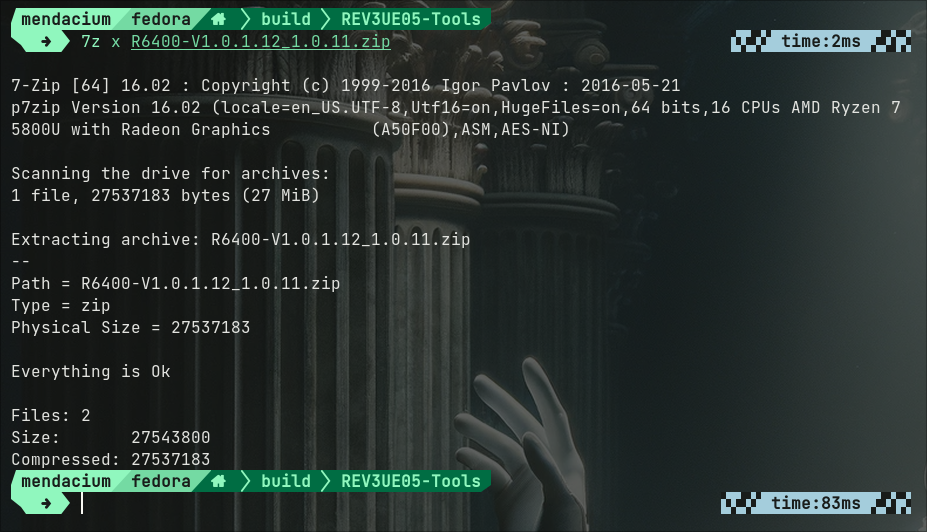
\includegraphics[width=0.5\linewidth]{"pictures/1.1 Extract.png"}\\
	Die Ausführung des Befehls \texttt{binwalk} mit der Option \texttt{--signature} auf die Datei \texttt{r6400-V1.0.1.12\_1.0.11.chk} liefert folgende Informationen über die Binärdatei der Firmware:\\
	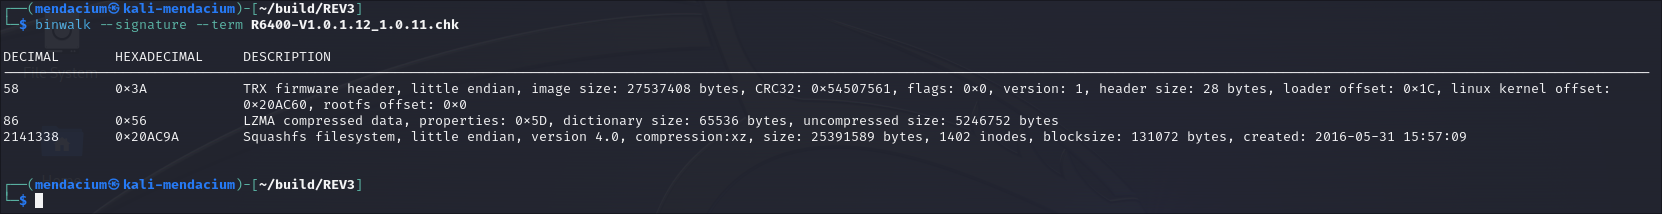
\includegraphics[width=1\linewidth]{"pictures/1.2 signature.png"}\\
	\begin{itemize}
		\item \textbf{TRX Firmware-Header:} Das Binärbild enthält einen TRX Firmware-Header, der häufig bei Firmware-Dateien für Router oder ähnliche Geräte verwendet wird. Er ist in Little-Endian-Format mit einer Größe des Images von 27.537.408 Bytes und enthält einen CRC32-Prüfsummenwert.\\
		Ein TRX-Header ist wie folgt aufgebaut:\\
		\begin{lstlisting}[language=c]
  0                   1                   2                   3   
 0 1 2 3 4 5 6 7 8 9 0 1 2 3 4 5 6 7 8 9 0 1 2 3 4 5 6 7 8 9 0 1 
+---------------------------------------------------------------+
|                     magic number ('HDR0')                     |
+---------------------------------------------------------------+
|                  length (header size + data)                  |
+---------------+---------------+-------------------------------+
|                       32-bit CRC value                        |
+---------------+---------------+-------------------------------+
|           TRX flags           |          TRX version          |
+-------------------------------+-------------------------------+
|                      Partition offset[0]                      |
+---------------------------------------------------------------+
|                      Partition offset[1]                      |
+---------------------------------------------------------------+
|                      Partition offset[2]                      |
+---------------------------------------------------------------+\end{lstlisting}
		Das Firmware-Image hat nicht wirklich einen Bootloader im klassischen Sinne. Der "loader offset" zeigt auf \textbf{0x1C} und es handelt sich dabei um einen LZMA-Loader, dieser startet einen selbst-entpackenden Kernel und somit die Firmware.
		Betrachtet man die Stelle \textbf{0x1C} ("loader offset"), so findet man zu Beginn einen String "\textbf{U12H332T00\_NETGEAR}"(radare2 visual mode). Dieser string gibt die Board ID an:\\
		\includegraphics[width=0.7\linewidth]{"pictures/1.2.1 bootloader"}
		
		\item \textbf{LZMA komprimierte Daten:} Der LZMA-komprimierte Teil (Lempel-Ziv-Markov-Kettenalgorithmus) im Header gibt Informationen über die Wortbuchgröße (65536 Bytes) und die unkomprimierte Datengröße des LZMA-Teils (5246752 Bytes). Die Daten sind vermutlich ausführerbarer Code für einen Kernel, welche zuerst dekomprimiert und anschließend ausgeführt werden. Dies ist der Start der Firmware.
		
		\item \textbf{Squashfs-Dateisystem:} Das Binärbild umfasst ein Squashfs-Dateisystem. Squashfs ist ein komprimiertes, schreibgeschütztes Dateisystem für Linux. Die Version, der Kompressionstyp (xz), die Größe, die Anzahl der Inodes, die Blockgröße und das Erstellungsdatum werden ebenfalls angegeben.
		Das Erstellungsdatum des Squashfs-Dateisystems ist der 31. Mai 2016 um 15:57:09 Uhr.
	\end{itemize}
	
	\noindent\textbf{Extrahieren} der LZMA komprimierten Datei und des squashfs-Dateisystems:\\
	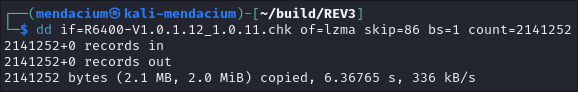
\includegraphics[width=0.4\linewidth]{"pictures/1.3 extract lzma.png"}
	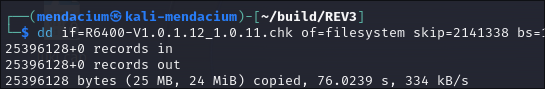
\includegraphics[width=0.4\linewidth]{"pictures/1.4 extract filesystem.png"}\\
	
	
	\noindent"\textbf{Mounten}" des Dateisystems in "\texttt{/mnt}":\\
	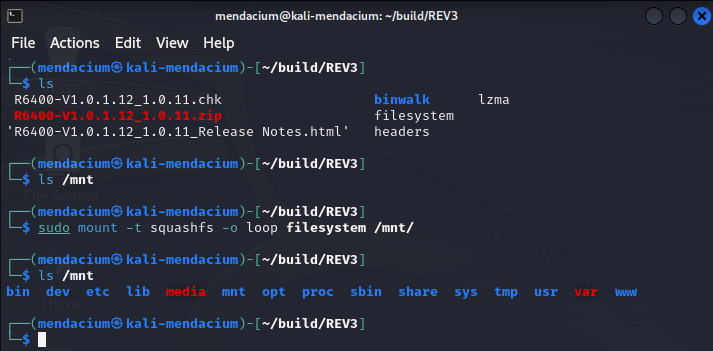
\includegraphics[width=0.4\linewidth]{"pictures/1.5 mount squashfs.png"}\\
	Suchen und finden der "httpd"-Binärdatei:\\
	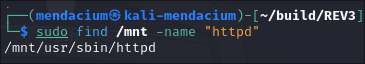
\includegraphics[width=0.4\linewidth]{"pictures/1.6 find httpd.png"}\\

	\pagebreak
	
	\subsection*{httpd}
	Informationen (radare2) über die Binärdatei:\\
	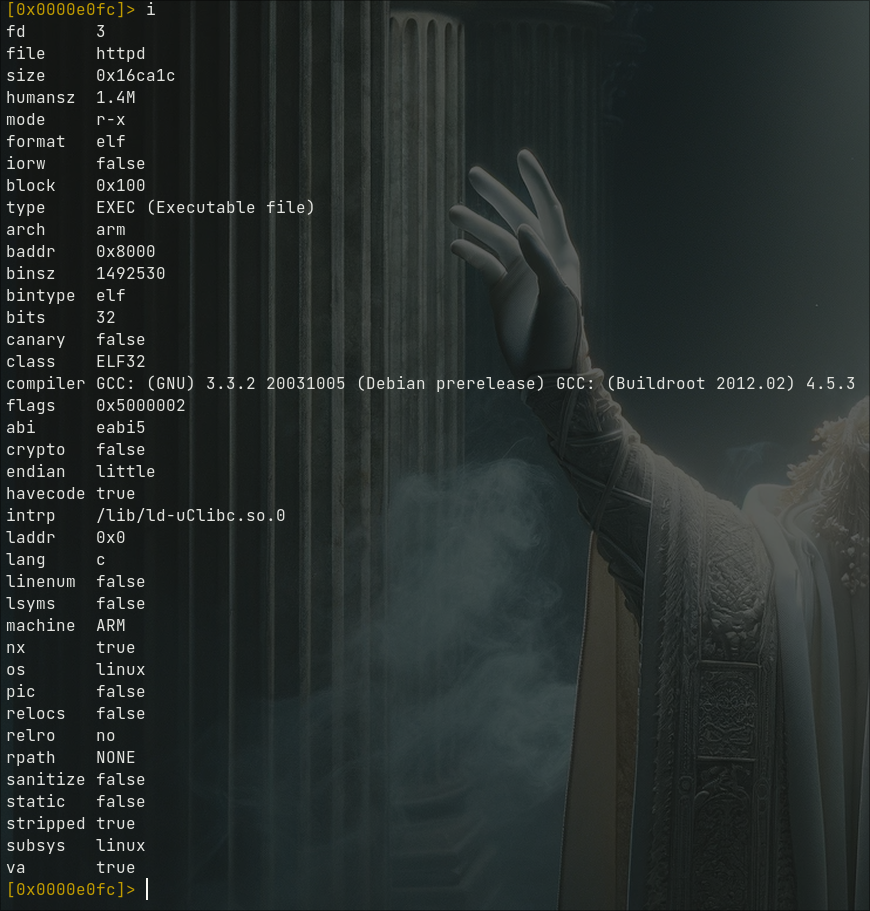
\includegraphics[width=0.4\linewidth]{"pictures/1.7 architecture, entry point.png"}\\
	Vergleicht man die httpd-Datei mit einer Datei aus der heruntergeladenen Open-Source/GPL \href{https://kb.netgear.com/2649/NETGEAR-Open-Source-Code-for-Programmers-GPL}{R6400-GPL\_V1.0.1.12\_1.0.11.zip}, sind gewisse Ähnlichkeiten festzustellen:\\
	\includegraphics[width=0.7\linewidth]{"pictures/1.8 httpd compare"}
	\begin{figure}[h]
		\centering
		\begin{minipage}{.5\textwidth}
			\centering
			\includegraphics[width=\linewidth]{"pictures/1.8 httpd compare downloaded"}
			\caption{downloaded}
		\end{minipage}%
		\begin{minipage}{.5\textwidth}
			\centering
			\includegraphics[width=\linewidth]{"pictures/1.8 httpd compare extracted"}
			\caption{extracted}
		\end{minipage}
	\end{figure}
	
	\pagebreak
	
	\noindent Alle Informationen scheinen gleich zu sein, lediglich die hash-Werte unterscheiden sich. Vergleicht man beide Binärdateien mit "radiff2", so sind ebenfalls wenig unterschiede festzustellen (womöglich durch die build-Umgebung):\\
	\includegraphics[width=0.7\linewidth]{"pictures/1.8 httpd compare2"}
	
	\subsection*{httpd - Vulnerability}
	Nach Recherche des Exploits wurde gefunden, dass commands unter \href{https://www.kb.cert.org/vuls/id/582384}{cgi-bin} ausgeführt werden. Dies ist ein guter Startpunkt um die interessanten Code-Stellen zu finden.\\
	In Ghidra kann zu Begin nach "cgi-bin/" gesucht werden:\\
	\includegraphics[width=1\linewidth]{"pictures/2.1 ghidra search"}\\
	Betrachtet man nun die Sucherergebnisse im Decompiler bekommt man ein gewisses Verständnis. Das print-statement in der obig-gezeigten Funktion lässt darauf schließen, dass "\texttt{param\_3}" die url ist:\\
	\includegraphics[width=0.7\linewidth]{"pictures/2.2 ghidra printf"}\\
	Eine genaue Analyse wie "\texttt{param\_3}" schluss-endlich ausgeführt wird, wurde nicht gemacht. Ein Umbenennen und Verfolgen der Variablen in Ghidra würde sehr sicher darauf hinführen, dass ein system-Aufruf mit "\texttt{acStack\_52c}" durchgeführt wird. Der Wert in acStack\_52 steht in Zusammenhang mit dem input der url und wird ohne weitere Überprüfungen und Authentifizierung ausgeführt.\\
	Systemaufruf:\\
	\includegraphics[width=0.7\linewidth]{"pictures/2.2 ghidra system"}\\

	\pagebreak
	
	Dekompilierte Funktion:\\
	\begin{lstlisting}[language=c]
undefined4 FUN_00033e0c(char *param_1,int param_2,char *param_3,int param_4)

{
	__pid_t _Var1;
	int iVar2;
	FILE *pFVar3;
	char *pcVar4;
	char *pcVar5;
	char *pcVar6;
	char *param3;
	size_t sVar7;
	undefined4 uVar8;
	uint uVar9;
	char *__s;
	char acStack_2052c [65536];
	char acStack_1052c [65536];
	char acStack_52c [512];
	char local_32c [256];
	char local_22c [256];
	undefined auStack_12c [64];
	char acStack_ec [64];
	char acStack_ac [64];
	undefined auStack_6c [32];
	undefined auStack_4c [16];
	char acStack_3c [16];
	int aiStack_2c [2];
	
	_Var1 = fork();
	if (_Var1 != 0) {
		if (0 < _Var1) {
			waitpid(_Var1,aiStack_2c,0);
		}
		return 0;
	}
	_Var1 = fork();
	if (_Var1 != 0) goto LAB_00034638;
	iVar2 = acosNvramConfig_match("ntgr_cgi_debug_msg","1");
	if (iVar2 != 0) {
		printf("\r\n###############%s(%d)url=%s,method=%d\r\n","netgear_commonCgi",0x3b,param_3,param_4)
		;
	}
	pFVar3 = fopen("/tmp/var/readydropd.conf","r");
	if (pFVar3 == (FILE *)0x0) {
		system("cp -f /www/cgi-bin/readydropd.conf /tmp/var/");
		iVar2 = acosNvramConfig_match("ntgr_cgi_debug_msg","1");
		if (iVar2 != 0) {
			puts("\r\n###################copy readydropd.conf\r");
		}
	}
	else {
		fclose(pFVar3);
	}
	pcVar4 = strstr(param_3,"cgi-bin");
	if (pcVar4 != (char *)0x0) {
		iVar2 = acosNvramConfig_match("ntgr_cgi_debug_msg","1");
		if (iVar2 != 0) {
			printf("\r\n##########%s(%d)\r\n","netgear_commonCgi",0x4c);
		}
		pcVar5 = strchr(pcVar4,0x3f);
		if (pcVar5 == (char *)0x0) {
			iVar2 = acosNvramConfig_match("ntgr_cgi_debug_msg","2");
			if (iVar2 != 0) {
				printf("\r\n##########%s(%d)\r\n","netgear_commonCgi",99);
			}
			pcVar6 = strchr(pcVar4,0x2f);
			__s = pcVar6 + 1;
			param3 = strchr(__s,0x2f);
			memset(acStack_ac,0,0x40);
			pcVar5 = pcVar6;
			if (pcVar6 != (char *)0x0) {
				pcVar5 = (char *)0x1;
			}
			if (param3 == (char *)0x0 || pcVar6 == (char *)0x0) {
				if (param3 == (char *)0x0) {
					uVar9 = (uint)pcVar5 & 1;
				}
				else {
					uVar9 = 0;
				}
				if (uVar9 != 0) {
					strcpy(acStack_ac,__s);
				}
			}
			else {
				strncpy(acStack_ac,__s,(size_t)(param3 + (-1 - (int)pcVar6)));
				iVar2 = acosNvramConfig_match("ntgr_cgi_debug_msg","2");
				if (iVar2 != 0) {
					printf("\r\n#############tmp1=%s,tmp2=%s,tmp3=%s,cgi=%s\r\n",pcVar4,pcVar6,param3,
					acStack_ac);
				}
				pcVar4 = local_32c;
				strcpy(pcVar4,param3);
				iVar2 = acosNvramConfig_match("ntgr_cgi_debug_msg","2");
				if (iVar2 != 0) {
					pcVar5 = "\r\n###############%s(%d)path_info=%s\r\n";
					uVar8 = 0x6e;
					goto LAB_000340e8;
				}
			}
		}
		else {
			iVar2 = acosNvramConfig_match("ntgr_cgi_debug_msg","1");
			if (iVar2 != 0) {
				printf("\r\n##########%s(%d)\r\n","netgear_commonCgi",0x50);
			}
			pcVar5 = strchr(pcVar4,0x3f);
			iVar2 = acosNvramConfig_match("ntgr_cgi_debug_msg","1");
			if (iVar2 != 0) {
				printf("\r\n#############%s(%d)tmp1=%s,tmp2=%s\r\n","netgear_commonCgi",0x53,pcVar4,
				pcVar5 + 1);
			}
			strcpy(local_22c,pcVar5 + 1);
			iVar2 = acosNvramConfig_match("ntgr_cgi_debug_msg","2");
			if (iVar2 != 0) {
				printf("\r\n###############%s(%d)query_string=%s\r\n","netgear_commonCgi",0x56,local_22c);
			}
			pcVar6 = strchr(param_3,0x2f);
			if (pcVar6 != (char *)0x0) {
				pcVar4 = acStack_ac;
				memset(pcVar4,0,0x40);
				strncpy(pcVar4,pcVar6 + 1,(size_t)(pcVar5 + (-1 - (int)pcVar6)));
				iVar2 = acosNvramConfig_match("ntgr_cgi_debug_msg","2");
				if (iVar2 != 0) {
					pcVar5 = "\r\n###############%s(%d)cgi_name=%s\r\n";
					uVar8 = 0x5d;
					LAB_000340e8:
					printf(pcVar5,"netgear_commonCgi",uVar8,pcVar4);
				}
			}
		}
	}
	if (param_4 == 0) {
		pcVar4 = "GET";
		LAB_00034150:
		strcpy(acStack_3c,pcVar4);
	}
	else {
		if (param_4 == 1) {
			pcVar4 = "POST";
			goto LAB_00034150;
		}
		if (param_4 == 2) {
			pcVar4 = "OPTIONS";
			goto LAB_00034150;
		}
	}
	iVar2 = acosNvramConfig_match("ntgr_cgi_debug_msg","2");
	if (iVar2 != 0) {
		printf("\r\n###############%s(%d)request_method=%s\r\n","netgear_commonCgi",0x82,acStack_3c);
	}
	if (local_32c[0] != '\0') {
		setenv("PATH_INFO",local_32c,1);
	}
	iVar2 = acosNvramConfig_match("ntgr_cgi_debug_msg","2");
	if (iVar2 != 0) {
		pcVar4 = getenv("PATH_INFO");
		printf("\r\n###############%s(%d)PATH_INFO=%s\r\n","netgear_commonCgi",0x88,pcVar4);
	}
	setenv("LD_LIBRARY_PATH","/usr/lib",1);
	iVar2 = acosNvramConfig_match("ntgr_cgi_debug_msg","2");
	if (iVar2 != 0) {
		pcVar4 = getenv("LD_LIBRARY_PATH");
		printf("\r\n###############%s(%d)LD_LIBRARY_PATH=%s\r\n","netgear_commonCgi",0x8c,pcVar4);
	}
	setenv("REQUEST_METHOD",acStack_3c,1);
	iVar2 = acosNvramConfig_match("ntgr_cgi_debug_msg","2");
	if (iVar2 != 0) {
		pcVar4 = getenv("REQUEST_METHOD");
		printf("\r\n###############%s(%d)REQUEST_METHOD=%s\r\n","netgear_commonCgi",0x90,pcVar4);
	}
	if (local_22c[0] != '\0') {
		setenv("QUERY_STRING",local_22c,1);
	}
	iVar2 = strcmp(acStack_3c,"POST");
	if (iVar2 == 0) {
		pFVar3 = fopen("/tmp/post_result","r");
		if (pFVar3 != (FILE *)0x0) {
			fclose(pFVar3);
			system("rm -f /tmp/post_result");
			iVar2 = acosNvramConfig_match("ntgr_cgi_debug_msg","2");
			if (iVar2 != 0) {
				puts("\r\n##########del post ############\r");
			}
		}
		system("rm -f /tmp/post_data.txt");
		sleep(1);
		pFVar3 = fopen("/tmp/post_data.txt","w");
		if (pFVar3 != (FILE *)0x0) {
			fputs(param_1,pFVar3);
			fclose(pFVar3);
		}
		pcVar4 = "/www/cgi-bin/%s > /tmp/post_result < /tmp/post_data.txt";
	}
	else {
		iVar2 = strcmp(acStack_3c,"OPTIONS");
		if (iVar2 == 0) {
			pFVar3 = fopen("/tmp/options_result","r");
			if (pFVar3 != (FILE *)0x0) {
				fclose(pFVar3);
				system("rm -f /tmp/options_result");
				iVar2 = acosNvramConfig_match("ntgr_cgi_debug_msg","2");
				if (iVar2 != 0) {
					puts("\r\n##########del option ############\r");
				}
			}
			pcVar4 = "/www/cgi-bin/%s > /tmp/options_result";
		}
		else {
			pFVar3 = fopen("/tmp/cgi_result","r");
			if (pFVar3 != (FILE *)0x0) {
				fclose(pFVar3);
				system("rm -f /tmp/cgi_result");
				iVar2 = acosNvramConfig_match("ntgr_cgi_debug_msg","2");
				if (iVar2 != 0) {
					puts("\r\n##########delete /tmp/cgi_result ############\r");
				}
			}
			pcVar4 = "/www/cgi-bin/%s > /tmp/cgi_result";
		}
	}
	sprintf(acStack_52c,pcVar4,acStack_ac);
	system(acStack_52c);
	memset(acStack_ec,0,0x40);
	memset(auStack_12c,0,0x40);
	memset(auStack_6c,0,0x20);
	memset(auStack_4c,0,0x10);
	iVar2 = acosNvramConfig_match("ntgr_cgi_debug_msg","1");
	if (iVar2 != 0) {
		printf("\r\n###############%s(%d)\r\n","netgear_commonCgi",200);
	}
	iVar2 = strcmp(acStack_3c,"POST");
	if (iVar2 == 0) {
		pcVar4 = "/tmp/post_result";
	}
	else {
		iVar2 = strcmp(acStack_3c,"OPTIONS");
		if (iVar2 == 0) {
			pcVar4 = "/tmp/options_result";
		}
		else {
			pcVar4 = "/tmp/cgi_result";
		}
	}
	pFVar3 = fopen(pcVar4,"r");
	if (pFVar3 != (FILE *)0x0) {
		iVar2 = acosNvramConfig_match("ntgr_cgi_debug_msg","1");
		if (iVar2 != 0) {
			printf("\r\n###############%s(%d)\r\n","netgear_commonCgi",0xd3);
		}
		while (pcVar4 = fgets(acStack_1052c,0xffff,pFVar3), pcVar4 != (char *)0x0) {
			iVar2 = acosNvramConfig_match("ntgr_cgi_debug_msg","1");
			if (iVar2 != 0) {
				printf("\r\n###############%s(%d)\r\n","netgear_commonCgi",0xd7);
			}
			pcVar4 = strstr(acStack_1052c,"Status:");
			if (pcVar4 == (char *)0x0) {
				strcat(acStack_2052c,acStack_1052c);
			}
			else {
				strcpy(acStack_ec,pcVar4 + 7);
				pcVar4 = strchr(acStack_ec,10);
				if (pcVar4 != (char *)0x0) {
					*pcVar4 = '\0';
				}
				iVar2 = acosNvramConfig_match("ntgr_cgi_debug_msg","2");
				if (iVar2 != 0) {
					printf("\r\n###############%s(%d)status=%s\r\n","netgear_commonCgi",0xdf,acStack_ec);
				}
				sprintf(acStack_2052c,"HTTP/1.1%s\r\n",acStack_ec);
			}
		}
		fclose(pFVar3);
	}
	strcat(acStack_2052c,"\r\n");
	iVar2 = acosNvramConfig_match("ntgr_cgi_debug_msg","1");
	if (iVar2 != 0) {
		printf("\r\n###############%s(%d)http_hdr=%s\r\n","netgear_commonCgi",0x114,acStack_2052c);
	}
	sVar7 = strlen(acStack_2052c);
	FUN_0000f27c(param_2,acStack_2052c,sVar7);
	iVar2 = acosNvramConfig_match("ntgr_cgi_debug_msg","2");
	if (iVar2 != 0) {
		printf("\r\n######======######%s(%d)\r\n","netgear_commonCgi",0x118);
	}
	LAB_00034638:
	/* WARNING: Subroutine does not return */
	exit(0);
}

\end{lstlisting}
	
	
	
	\label{LastPage}
	
\end{document}